\documentclass[12pt, a4paper]{article}

\usepackage{amsmath, amssymb, amsthm}
\usepackage{geometry}
\usepackage{booktabs}
\usepackage{array}
\usepackage{hyperref}
\usepackage{xcolor}
\usepackage{tcolorbox}
\usepackage{enumitem}
\usepackage{parskip}
\usepackage{tikz}
\usetikzlibrary{arrows.meta, positioning, calc}

\geometry{margin=2.5cm}

\newif\ifstudentmode
\studentmodefalse
\ifx\studentflag\undefined\else\studentmodetrue\fi

\newcommand{\sol}[2][6cm]{%
  \ifstudentmode\underline{\hspace{#1}}\else{#2}\fi}

\definecolor{mainblue}{RGB}{30, 100, 180}
\definecolor{boxbg}{RGB}{235, 243, 255}
\definecolor{notebg}{RGB}{255, 248, 230}
\definecolor{warnbg}{RGB}{255, 235, 235}
\definecolor{greenbg}{RGB}{230, 255, 235}

\tcbuselibrary{skins, breakable}

\newtcolorbox{resultbox}{colback=boxbg,colframe=mainblue,boxrule=1.2pt,arc=4pt,
  title={Result},fonttitle=\bfseries\color{white},coltitle=white,
  attach boxed title to top left={yshift=-2mm,xshift=4mm},
  boxed title style={colback=mainblue,arc=3pt}}

\newtcolorbox{notebox}{colback=notebg,colframe=orange!70!black,
  boxrule=1pt,arc=4pt,left=4pt,right=4pt}

\newtcolorbox{warnbox}{colback=warnbg,colframe=red!60!black,
  boxrule=1pt,arc=4pt,left=4pt,right=4pt}

\theoremstyle{definition}
\newtheorem{example}{Example}[section]

\begin{document}

\begin{center}
  {\LARGE \textbf{Section 4.3: Early Stopping}} \\[0.3em]
  {\large\itshape Stop Training Before the Network Overfits} \\[0.5em]
  {\large AI Class --- Lecture Notes}%
  \ifstudentmode\quad{\normalsize\color{gray}[Student Copy]}\fi
\end{center}

\vspace{1em}\hrule\vspace{1.5em}

% ══════════════════════════════════════════════════════════════════════════════
\section{The Idea}

Regularisation (L1/L2) and dropout modify the network or the loss to slow
down overfitting.  \textbf{Early stopping} is simpler: just
\emph{watch the validation loss and stop when it starts getting worse}.

The training loss will always decrease if we keep training long enough ---
the network has enough capacity to memorise the data.
The validation loss, however, shows us how well the network will perform on
\emph{new} data.  When it starts to rise, we have found the sweet spot.

% ══════════════════════════════════════════════════════════════════════════════
\section{How It Works}

\begin{enumerate}
  \item Split the data into \textbf{training set} and \textbf{validation set}
        (e.g.\ 80\,\% / 20\,\%).
  \item At the end of every epoch, evaluate the loss on both sets.
  \item Keep a copy of the weights at the epoch with the
        \textbf{lowest validation loss} so far.
  \item If the validation loss has not improved for $k$ consecutive epochs
        (the \textbf{patience}), stop training and restore the best weights.
\end{enumerate}

\begin{resultbox}
\textbf{Early stopping requires no modification to the network or loss
function.}
It is the cheapest regulariser available.
\end{resultbox}

% ══════════════════════════════════════════════════════════════════════════════
\section{Illustrative Loss Table}

\begin{center}
\renewcommand{\arraystretch}{1.4}
\begin{tabular}{cccp{5cm}}
\toprule
Epoch & Train loss & Val loss & Note \\
\midrule
1  & 0.820 & 0.810 & Both high --- still learning \\
2  & 0.650 & 0.645 & Improving together \\
3  & 0.480 & 0.475 & Improving together \\
4  & 0.330 & 0.338 & \\
5  & 0.210 & 0.240 & \\
\rowcolor{greenbg!60}
6  & 0.140 & \textbf{0.220} & \textbf{Best validation loss so far} $\leftarrow$ save weights \\
7  & 0.090 & 0.231 & Val loss rising --- patience 1 \\
8  & 0.060 & 0.258 & Val loss rising --- patience 2 \\
9  & 0.042 & 0.289 & Val loss rising --- patience 3 \\
\rowcolor{warnbg!60}
10 & 0.031 & 0.320 & \textbf{Stop.} Restore epoch-6 weights \\
\bottomrule
\end{tabular}
\end{center}

With patience $= 4$, training stops at epoch 10 and the weights from
epoch 6 are restored.  The training loss at epoch 10 is $0.031$ ---
far lower than at epoch 6 --- but the model at epoch 10 would perform
much worse on new data.

% ══════════════════════════════════════════════════════════════════════════════
\section{The Learning Curve}

\begin{center}
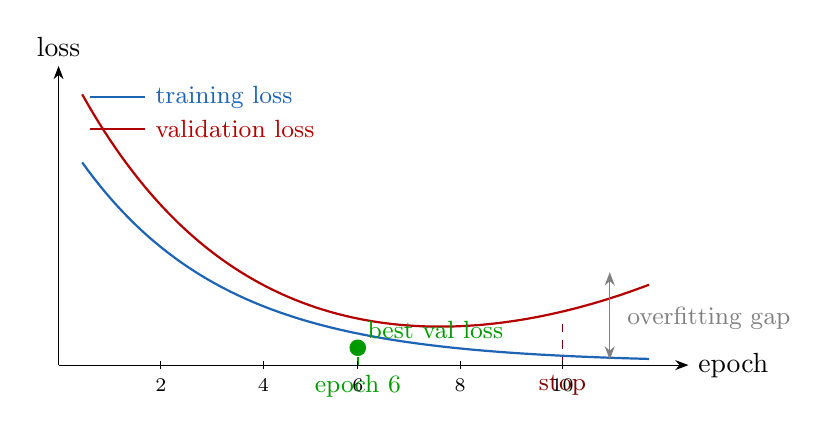
\begin{tikzpicture}[scale=1.0, >=Stealth]
  \draw[->] (0,0) -- (8,0) node[right] {epoch};
  \draw[->] (0,0) -- (0,3.8) node[above] {loss};

  % Training loss (monotone decrease)
  \draw[thick, mainblue, domain=0.3:7.5, samples=100]
    plot (\x, {3.0*exp(-0.55*\x) + 0.03});

  % Validation loss (U-shaped, minimum around epoch 6)
  \draw[thick, red!70!black, domain=0.3:7.5, samples=100]
    plot (\x, {3.0*exp(-0.55*\x) + 0.22 + 0.055*(\x-3.8)^2});

  % Best point (epoch 6 ≈ x=3.8 in scaled coords)
  \draw[dashed, green!60!black, thick] (3.8,0) -- (3.8,0.22);
  \fill[green!60!black] (3.8,0.22) circle (3pt);
  \node[above right, green!60!black, font=\small] at (3.8,0.22) {best val loss};
  \node[below, green!60!black, font=\small] at (3.8,0) {epoch 6};

  % Stop point
  \draw[dashed, red!50!black] (6.4,0) -- (6.4,0.57);
  \node[below, red!50!black, font=\small] at (6.4,0) {stop};

  % Gap annotation
  \draw[<->, gray] (7.0, 0.07) -- (7.0, 1.18);
  \node[right, gray, font=\small] at (7.1, 0.6) {overfitting gap};

  % Legend
  \draw[thick, mainblue]        (0.4,3.4) -- (1.1,3.4) node[right,font=\small] {training loss};
  \draw[thick, red!70!black]    (0.4,3.0) -- (1.1,3.0) node[right,font=\small] {validation loss};

  % Axis ticks
  \foreach \e/\x in {2/1.3, 4/2.6, 6/3.8, 8/5.1, 10/6.4}
    \draw (\x,0.05) -- (\x,-0.05) node[below,font=\scriptsize] {\e};
\end{tikzpicture}
\end{center}

% ══════════════════════════════════════════════════════════════════════════════
\section{Choosing Patience}

\begin{center}
\renewcommand{\arraystretch}{1.3}
\begin{tabular}{lll}
\toprule
Patience $k$ & Behaviour & Risk \\
\midrule
Very small (1--2) & Stops very early & May stop before true minimum \\
Moderate (5--10)  & Good default     & Balanced \\
Large (20+)       & Trains long      & May not prevent overfitting \\
\bottomrule
\end{tabular}
\end{center}

\begin{warnbox}
\textbf{Validation set must not be used for any other decisions}
(e.g.\ tuning $\lambda$ or $p$) once it is used for early stopping.
If you tune hyperparameters on the validation set, use a separate
\textbf{test set} to report the final performance.
\end{warnbox}

\begin{notebox}
\textbf{PyTorch.}
PyTorch has no built-in early stopping, but it is easy to implement
manually.  See \texttt{code\_examples.py} for a clean loop that saves
the best checkpoint and restores it at the end.
\end{notebox}

\end{document}
